% \pgfdeclareimage[width=2cm]{enclave}{icons/enclave}
% \pgfdeclareimage[width=2cm]{enclave-yellow}{icons/sgx_red}
% \pgfdeclareimage[width=2cm]{enclave-red}{icons/sgx_yellow}
% \pgfdeclareimage[width=2cm]{server}{icons/server_contoured}
% \pgfdeclareimage[width=2cm]{blockchain}{icons/blockchain}
% \pgfdeclareimage[width=2cm]{user}{icons/persons/user/user}
% \pgfdeclareimage[width=2cm]{attacker}{icons/persons/burglar}
% \pgfdeclareimage[width=1cm]{phone}{icons/smartphone}
% \pgfdeclareimage[width=2cm]{computer}{icons/devices/client}

% \pgfdeclareimage[width=2cm]{memory}{icons/computerpack/013-ram}
% \pgfdeclareimage[width=1.4cm]{gpu}{icons/computerpack/002-vga}
% \pgfdeclareimage[width=1.4cm]{mouse}{icons/computerpack/017-mouse}
% \pgfdeclareimage[width=1.4cm]{keyboard}{icons/computerpack/024-keyboard}
% \pgfdeclareimage[width=1.4cm]{screen}{icons/computerpack/018-monitor-2}
% \pgfdeclareimage[width=1.4cm]{lan}{icons/computerpack/023-lan}
% \pgfdeclareimage[width=1.4cm]{lanred}{icons/computerpack/023-lan-red}

% \definecolor{col1}{RGB}{170, 72, 59}
% \definecolor{col2}{RGB}{170,114, 59}
% \definecolor{col3}{RGB}{ 38, 93,105}
% \definecolor{col4}{RGB}{ 44,127, 66}

\definecolor{col1}{HTML}{4398D1}
\definecolor{col2}{HTML}{FF4842}
\definecolor{col3}{RGB}{ 38, 93,105}
\definecolor{col4}{RGB}{ 44,127, 66}

\definecolor{greenc}{HTML}{64c37d}
\definecolor{redc}{HTML}{e13957}

\ifstandalone
    \newcommand{\icon}[1]{../icons/#1}
\else
    \newcommand{\icon}[1]{images/icons/#1}
\fi

\newcommand{\imgmemory}{
\includegraphics[width=2.0cm]{\icon{computerpack/013-ram}}}
\newcommand{\imggpu}{
\includegraphics[width=1.4cm]{\icon{computerpack/002-vga}}}
\newcommand{\imggpusmall}{
\includegraphics[width=1.0cm]{\icon{computerpack/002-vga}}}
\newcommand{\imgmouse}{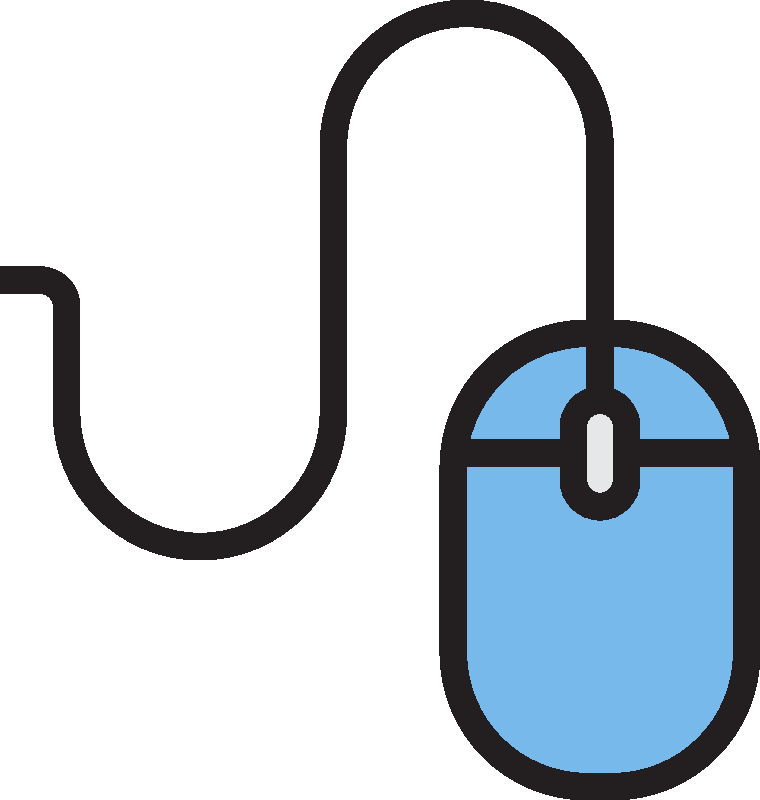
\includegraphics[width=1.4cm]{\icon{computerpack/017-mouse}}}
\newcommand{\imgkeyboard}{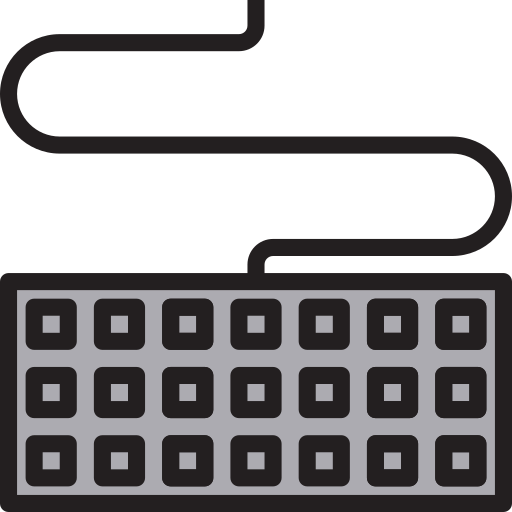
\includegraphics[width=1.4cm]{\icon{computerpack/024-keyboard}}}
\newcommand{\imgscreen}{\includegraphics[width=1.4cm]{\icon{computerpack/018-monitor}}}
\newcommand{\imglan}{
\includegraphics[width=1.4cm]{\icon{computerpack/023-lan}}}
\newcommand{\imglanred}{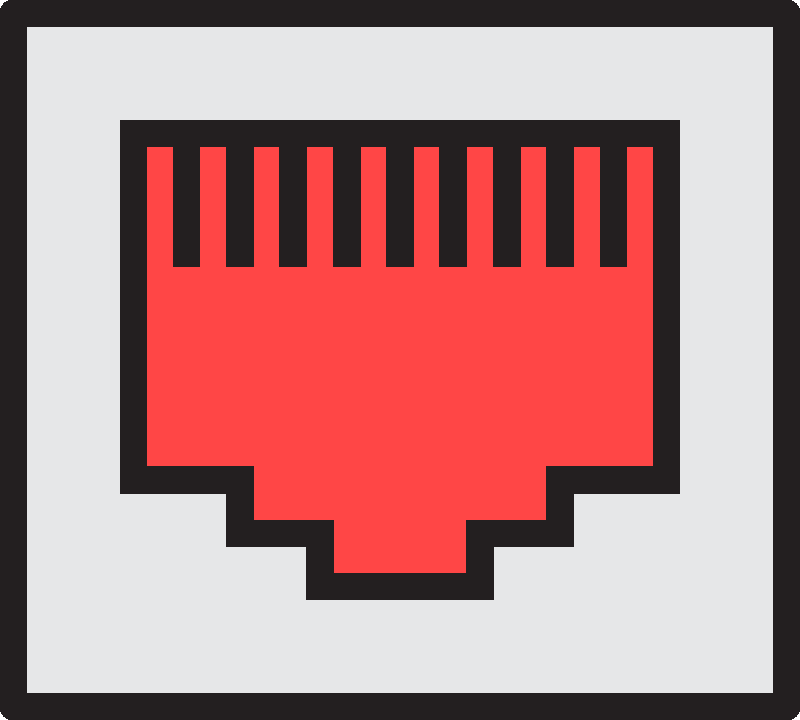
\includegraphics[width=1.4cm]{\icon{computerpack/023-lan-red}}}
\newcommand{\imgcpu}{
\includegraphics[width=1.4cm]{\icon{computerpack/034-cpu}}}
\newcommand{\imgcpusmall}{
\includegraphics[width=1.0cm]{\icon{computerpack/034-cpu}}}

\newcommand{\imgdisplay}{
\includegraphics[height=1.4cm]{\icon{computerpack/021-mobile}}}
\newcommand{\imgdisplaysmall}{
\includegraphics[height=1.0cm]{\icon{computerpack/021-mobile}}}
\newcommand{\imgsim}{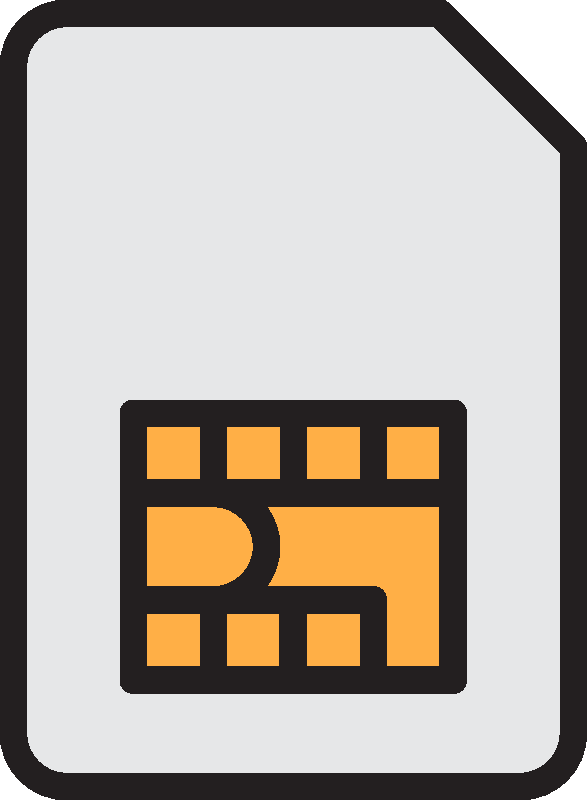
\includegraphics[height=1.4cm]{\icon{computerpack/008-sim-card}}}
\newcommand{\imgsimsmall}{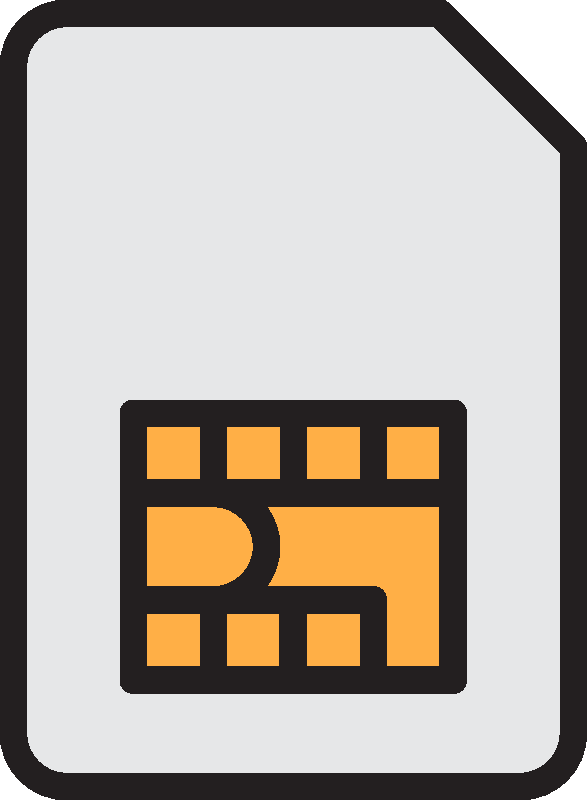
\includegraphics[height=1.0cm]{\icon{computerpack/008-sim-card}}}
\newcommand{\imgsd}{
\includegraphics[height=1.4cm]{\icon{computerpack/011-sd-card}}}
\newcommand{\imgsdsmall}{
\includegraphics[height=1.0cm]{\icon{computerpack/011-sd-card}}}
\newcommand{\imgcamera}{
\includegraphics[width=1.4cm]{\icon{computerpack/035-camera}}}
\newcommand{\imgcamerasmall}{
\includegraphics[width=1.0cm]{\icon{computerpack/035-camera}}}

\newcommand{\imgenclave}{\includegraphics[width=2.0cm]{\icon{enclave}}}
\newcommand{\imgenclavesmall}{\includegraphics[width=1.4cm]{\icon{enclave}}}
\newcommand{\imgenclavesmaller}{\includegraphics[width=1.0cm]{\icon{enclave}}}
\newcommand{\imgenenclavered}{\includegraphics[width=2.0cm]{\icon{sgx_red}}}
\newcommand{\imgenenclaveredsmall}{\includegraphics[width=1.0cm]{\icon{sgx_red}}}
\newcommand{\imguser}{
\includegraphics[height=2.0cm]{\icon{persons/user/user}}}
\newcommand{\imgusersmall}{
\includegraphics[height=1.4cm]{\icon{persons/user/user}}}
\newcommand{\imgattacker}{
\includegraphics[width=2.0cm]{\icon{persons/burglar}}}
\newcommand{\imgattackersmall}{
\includegraphics[height=1.4cm]{\icon{persons/burglar}}}
\newcommand{\imgcomputer}{
\includegraphics[width=2.0cm]{\icon{devices/client}}}

\newcommand{\imglock}{\includegraphics[width=0.3cm]{\icon{lock-icon}}}
\newcommand{\imglocklarge}{\includegraphics[width=0.5cm]{\icon{lock-icon}}}
\newcommand{\imgkeyyellow}{\includegraphics[width=0.5cm]{\icon{key-yellow}}}
\newcommand{\imgkeyred}{\includegraphics[width=0.5cm]{\icon{key-red}}}
\newcommand{\imgkeyblue}{\includegraphics[width=0.5cm]{\icon{key-blue}}}
\newcommand{\imgcertred}{\includegraphics[width=0.5cm]{\icon{certificate-red}}}
\newcommand{\imgcertyellow}{\includegraphics[width=0.5cm]{\icon{certificate-yellow}}}
\newcommand{\imgcertblue}{\includegraphics[width=0.5cm]{\icon{certificate-blue}}}

\newcommand{\imgdevil}{\includegraphics[width=0.6cm]{\icon{devil}}}

\def\nameenclave{platform-wide enclave\xspace}
\def\Nameenclave{Platform-wide enclave\xspace}


\newcommand{\sphw}[0]{peripheral\xspace}
\newcommand{\Sphw}[0]{Peripheral\xspace}

\newcommand{\risc}{RISC-V\xspace}
\newcommand{\ce}{controller enclave\xspace}
\newcommand{\ces}{controller enclave\xspace}
\newcommand{\Ce}{Controller enclave\xspace}
\newcommand{\Ces}{Controller enclave\xspace}
\let\oldemph\app
\renewcommand{\app}{application enclave\xspace}
\newcommand{\App}{Application enclave\xspace}
\newcommand{\apps}{application enclaves\xspace}
\newcommand{\Apps}{Application enclaves\xspace}

\let\oldemph\name
\renewcommand{\name}{\textsc{PIE}\xspace}
\let\oldemph\tool
\renewcommand{\tool}{\textsc{\name{} API}\xspace}
\let\oldemph\device
\renewcommand{\device}{\textsc{Device}\xspace}